\documentclass{article} % For LaTeX2e
\usepackage{xr}
%\externaldocument{Appendix}


\usepackage{nips15submit_e,times}



%=========================================================
% Standard Packages
%=========================================================

\usepackage[numbers]{natbib}
\usepackage{hyperref}
\usepackage{url}
\usepackage{amsmath,amsthm,amsfonts,amssymb,mathtools, fancyvrb}
\usepackage{algorithm,algorithmic}
%\usepackage[noend]{,amssymb,amsfonts,amsmath}
%\usepackage[linesnumbered,ruled]{algorithm2e}
\usepackage{graphicx}
\usepackage{xcolor}
\usepackage{url}
\usepackage{bbold}
\usepackage{wrapfig}
\usepackage[footnotesize]{subfigure}
\usepackage{caption}
\captionsetup{labelfont=bf,font={small},format=plain}

%\graphicspath{{./plt/}}

\nipsfinalcopy

%=========================================================
% Stephan's Macros
%=========================================================

\newcommand{\be}{\begin{eqnarray}}
\newcommand{\ee}{\end{eqnarray}}
\newcommand{\n}{\nonumber \\}
\newcommand{\E}[1]{{\mathbb E} \left[#1\right]}
\newcommand*\colvec[1]{\begin{pmatrix}#1\end{pmatrix}}


%=========================================================
% Marius' Macros
%=========================================================

\newtheorem{theorem}{Theorem}
\newtheorem{problem}{Problem}
\newcommand{\sign}{{\text{sign}}}
\newcommand{\Log}{{\text{Logistic}}}
\newcommand{\w}{{\boldsymbol{w}}}
\newcommand{\x}{{\boldsymbol{x}}}
\newcommand{\y}{{\boldsymbol{y}}}
\newcommand{\vepsilon}{{\boldsymbol{\epsilon}}}
\newcommand{\comment}[1]{\textcolor{red}{{[#1]}}}
\newcommand{\CL}[1]{\textcolor{red}{CL: {#1}}}
\newcommand{\fix}{\marginpar{\textcolor{red}{FIX}}}
%=========================================================
%=========================================================


\DeclareMathOperator*{\argmin}{arg\,min}
\DeclareMathOperator*{\argmax}{arg\,max}

%%%%%%%HACKS%%%%%%%%%%%%%%%
\abovedisplayskip 5pt plus0pt minus0pt%
\belowdisplayskip \abovedisplayskip
\parskip .3pc
%\abovedisplayshortskip  0pt plus3pt%
%\belowdisplayshortskip  4pt plus3pt minus3pt%
%%%%%%%HACKS%%%%%%%%%%%%%%%


%=========================================================


%=========================================================

\VerbatimFootnotes
%=========================================================
\begin{document}

\title{Consistent Representations of Variable Length Peptides for Predicting Peptide-MHC Binding Affinity}

\author{
Giancarlo Kerg\\
Icahn School of Medicine at Mount Sinai \\
\texttt{gc@hammerlab.org} \\
\And
Kyunghyun Cho\\
New York University \\
\texttt{kyunghyun.cho@nyu.edu} \\
\And
Alex Rubinsteyn\\
Icahn School of Medicine at Mount Sinai \\
\texttt{alex@hammerlab.org} \\
\And
Tim O'Donnell\\
Icahn School of Medicine at Mount Sinai \\
\texttt{tim@hammerlab.org} \\
\And
Jeff Hammerbacher \\
Icahn School of Medicine at Mount Sinai  \\
\texttt{hammer@hammerlab.org}
}

\maketitle 
\vspace{-0.3cm}
%=========================================================


%=========================================================

%=========================================================


%=========================================================
\begin{abstract}
\vspace{-0.15cm}
Predicting the binding affinity between MHC proteins their peptide ligands is a key problem in T-cell vaccine design.  In this paper we focus only on peptide-MHC class I binding affinity prediction. A couple of fairly successful models have been produced as explained in \cite{cit1}. Most of those models use shallow neural networks models, and rely on fixed length peptide encoding. For MHC class I, most but not all peptides are of length 9, thus we face the challenge of encoding peptides of varying length via fixed length encoding. For shallow neural networks this has been achieved via 9mer-index-encoding. Fixed length encoding does not carry the full information of dataset. A natural candidate for handling varying length sequences are LSTMs. Its performance is however unexpectedly low compared to shallow neural network models. Even more surprising is the fact that LSTMs perform worse than shallow nets on non 9 mers, while performing almost equally on 9 mers. We will present a method that uses a convolutional filter before the information gets processed into the LSTM. This could be an essential building block for MHC class II binding prediction, as in the latter case the distribution of peptides length has much higher variance. 

\vspace{-0.2cm}

\end{abstract}
%=========================================================



%=========================================================
\section{Introduction}
%=========================================================
\vspace{-0.1cm}

\subsection{Background and motivation}

T-cell receptors (TCRs) and B-cell receptors (BCRs) scan cellular surfaces for non-self peptides and trigger an immune response upon detection. TCRs binding peptide - MHC class I are associated with cytotoxic T-cell response whereas TCRs binding peptide-MHC class I are associated with the recruitment of helper T-cells and alerting of B-cells. Improved understanding of immune epitope recognition will enhance the development of novel vaccines, diagnostics and therapeutics in treating infectious and autoimmune diseases, allergies and cancers.

In this paper we focus merely on peptide-MHC class I binding affinity prediction. Peptides are being presented by single letter amino acids as inputs. Predictions are made against a set of MHC class I molecules. Outputs consist of predicted IC50 binding affinity scores, indicating the likelihood of binding between a given peptide and a given MHC class I molecule. For convenience of training, outputs are log-transformed between 0 and 1.

%-------------------
\subsection{Dataset}

Two datasets were used from a recent paper studying the relationship between training data and peptide-MHC predictor accuracy. \cite{Kim_2014}. 
The training dataset (BD2009) contained entries from IEDB~\cite{Salimi_2012}
up to 2009, containing 56 human, 19 non-human primate and six mouse alleles. The test dataset (BLIND) contained IEDB entries from between 2010 and 2013 which did not overlap with BD2009 (Table~\ref{tab:datasets}).

\begin{table}[h!]
\centering
\begin{tabular}{l||cccc}
{} & Alleles &  IC50 Measurements & Expanded 9mers \\

BD2009 &     106 &                           137,654 &        470,170 \\
BLIND  &      53 &                           27,680 &         83,752 \\

\end{tabular}
\caption{Train (BD2009) and test (BLIND) dataset sizes.}
\label{tab:datasets}
\end{table}

Throughout this paper we will evaluate using {\bf AUC} "Area under the ROC curve", which estimates the probability that a ``strong binder'' peptide (affinity $\leq 500$nM) will be given a stronger predicted affinity than one whose ground truth affinity is $>500$nM. This performance metric was also used to evaluate the state-of-the-art model. 

\subsection{State-of-the-art}

Three major prediction methods have been added: 
\begin{itemize}
\item The first one being a SMM predictor based on amino acid similarity score martrices. 
\item The second one being a pan-allele neural network based predictor NetMHCpan, which is similar to NetMHC, but being trained on all MHC molecules simultaneously and thus allowing an extrapolation of binding affinities for underrepresented or missing MHC molecules. 
\item The third being an ensemble method approach combining NetMHC, SMM and CombLib if a trained predictor is available for the molecule. Otherwise, NetMHCpan is used. This choice was motivated by the expected predictive performance of the methods in decreasing order: Consensus $>$ NetMHC $>$ SMM $>$ NetMHCpan $>$ Comb-Lib. This ensemble method is currently considered to be the state-of-the-art and used by 'IEDB Recommended'.
\end{itemize}

Most methods are entirely sequence-based, despite potential advantages of structure-based methods. However one expects improvement of structural approaches with comparable or better performance to come.  

The reference model we are using for comparison is a shallow neural network, as this is the core model behind the state-of-the art ensemble approach. The shallow net we are using contains:
\begin{itemize}
  \item an embedding layer which transforms amino acids to learned vector representations
  \item a single hidden layer of size $10$ with $tanh$ nonlinearity
  \item a sigmoidal scalar output 
\end{itemize}

We noted that neither increasing the hidden layer size nor the depth of the network helps improving the performance.

%=========================================================
\subsection{Challenge of varying length peptide encoding}
%=========================================================
Generally there are two ways to encode peptide: "hotshot encoding" or "index encoding" followed by an embedding layer.
We chose the latter, due to better performance.\\

Most models such as shallow neural networks rely on fixed length peptide encoding. Encoding varying length peptide into fixed length peptide sequences is delicate as one might lose important information from the dataset. Padding with zeros the encoded peptide until reaching the maximal peptide length within the dataset, does not work well as the last amino acid position then has varying positions. \\

For shallow neural network models one has come up with the so-called {\bf"9mer-index-encoding"}: it
uses fixed length 9mer inputs which requires peptides of other lengths to be transformed into multiple 9mers. Shorter peptides are mapped onto 9mer query peptides by introducing a sentinel ``X'' at every possible position, whereas longer peptides are cut into multiple 9mers by removing consecutive stretches of residues. The predicted affinity for a non-9mer peptide is the geometric mean of the predictions for the generated 9mers. When $n$ training samples derive from a single non-9mer sequence then their weights are adjusted to $1/n$. 

\subsection{Label encoding}

We map IC50 concentrations onto regression targets between 0.0 and 1.0 using the same scheme as NetMHC, $y = 1.0 - \textrm{min}(1.0, \log_{50000}(\textrm{IC50}))$.
%-------------------

%=========================================================
\section{Long Short-Term Memory models}
%=========================================================
\subsection{Motivation}

LSTM models are a natural candidate for this problem as they are able to handle sequences of varying length without having to rely on some encoding scheme such as "9mer-index-encoding". Despite giving reasonable performance, "9mer-index-encoding" does not use the full power of the dataset. 

\subsection{LSTM vs simple shallow nets}

The first thing to try is to evaluate the performance of a LSTM against the simple shallow net reference model. We have found that it is most beneficial to have a bidirectional LSTM model. In terms of hyperparameters, the most important one for LSTM models is the learning rate, followed by the hidden size \cite{cit2}. The learning rate can be tuned independently of other parameters, thus in order to save computing time, one can tune learning rate with very small models, and thus extrapolate to larger models.

Three-fold cross validation on the training set was used to select the hyper-parameters. We selected the following model:
\begin{itemize}
  \item batch size of 16	
  \item 32 output dimensions for the amino acid vector embedding
  \item the hidden layer size of the LSTM being $50$
  \item bidirectional LSTM with common embedding layer, concatenated outputs, and no internal dropouts.
  \item the concatenated outputs are followed by a single dense sigmoid output with dropout rate $0.25$.
  \item Adaptive Moment Estimation (Adam) as optimization procedure.
  \item learning rate equal to $0.01* 1/(1+N)^2$, with $N$ being the number of epochs.  
\end{itemize}

Less aggressive learning rate decays were found to lead to overfitting, no matter how we tune the various dropout parameters. We also found that deeper models don't improve performance. 

Despite being able to handle sequences of varying length, our LSTM performs worse than the shallow neural net reference model. \\

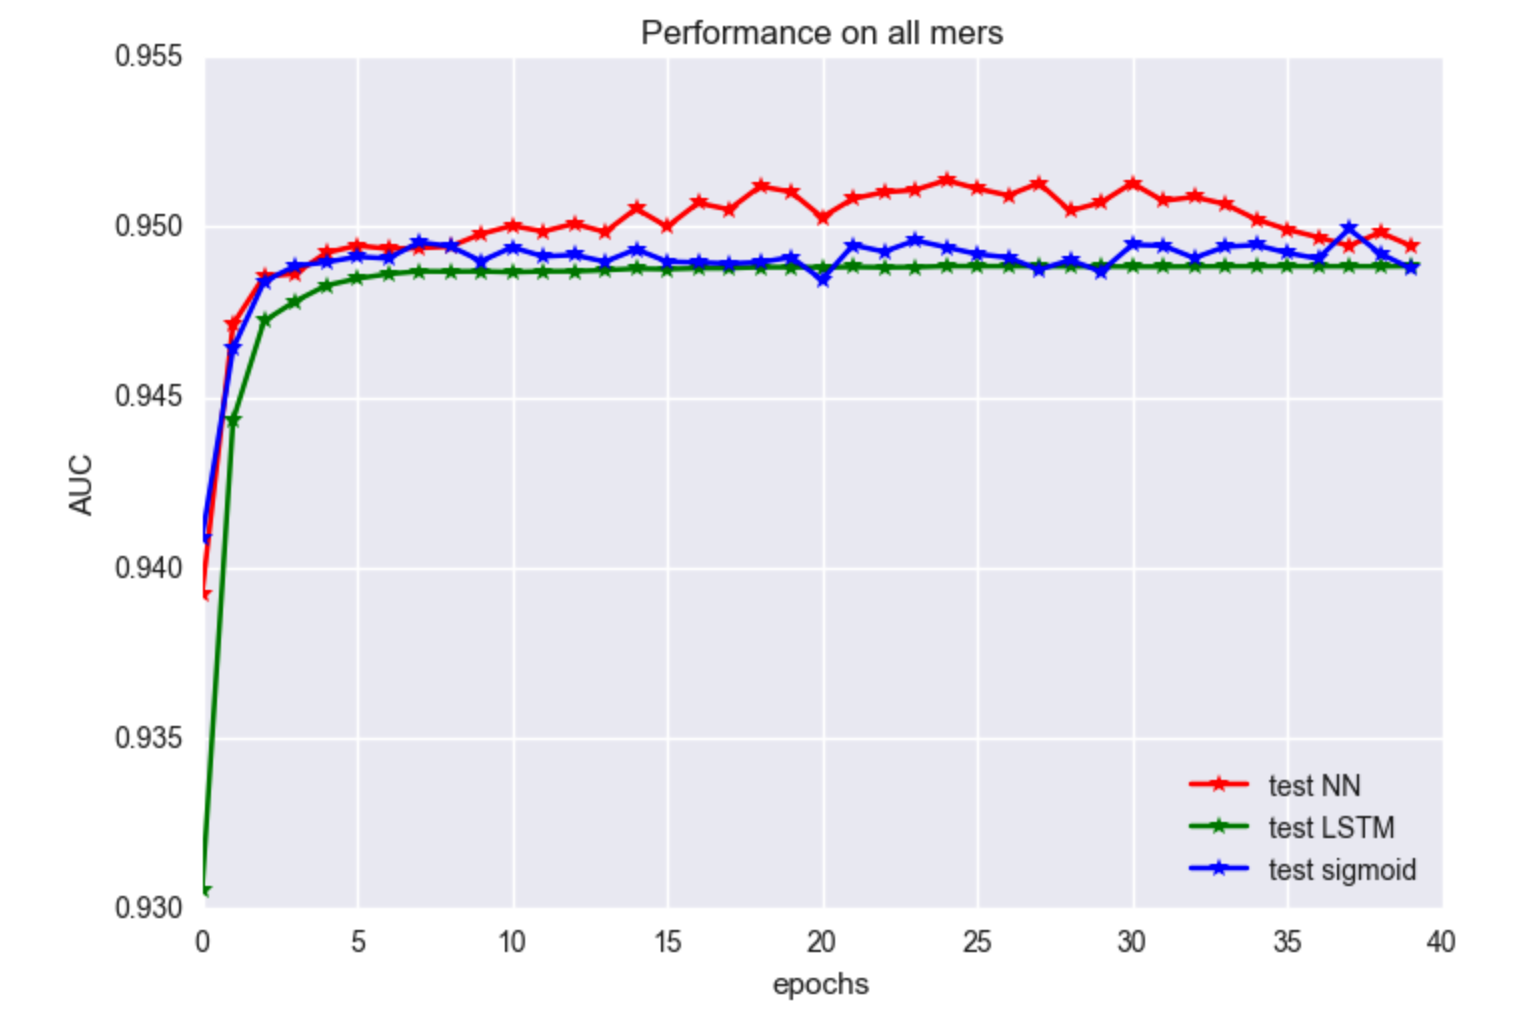
\includegraphics[scale = 0.17]{LSTM_vs_FFN_vs_sigmoid.png}
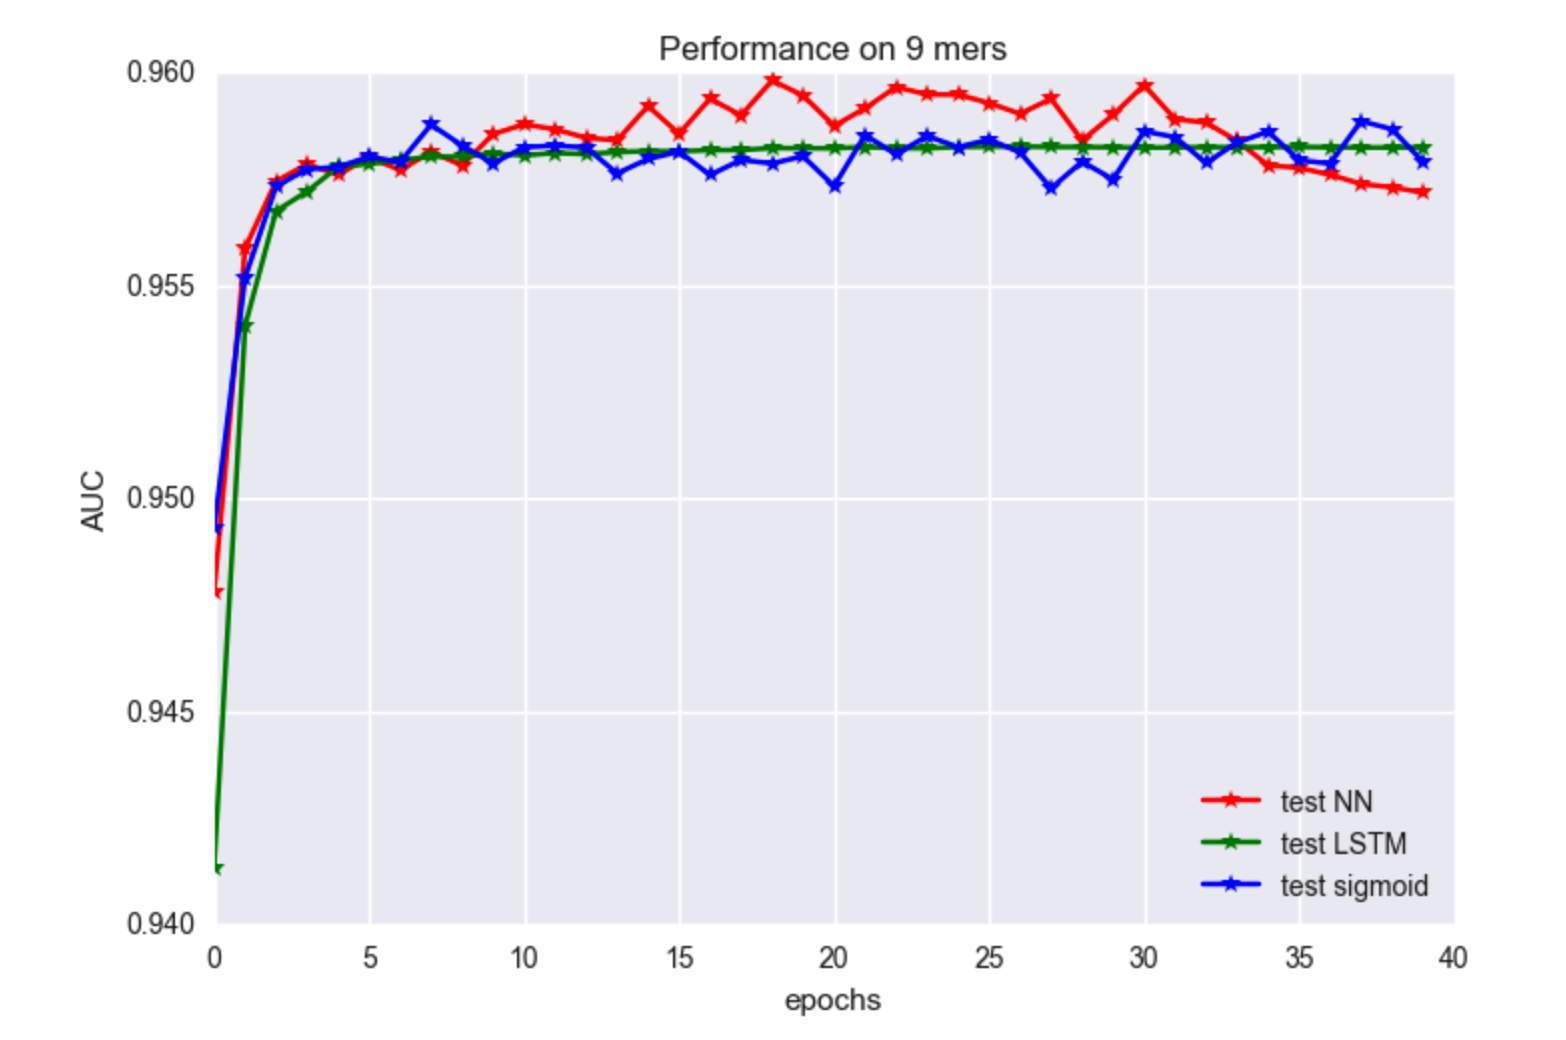
\includegraphics[scale = 0.17]{LSTM_vs_FFN_vs_sigmoid_9mers.png}
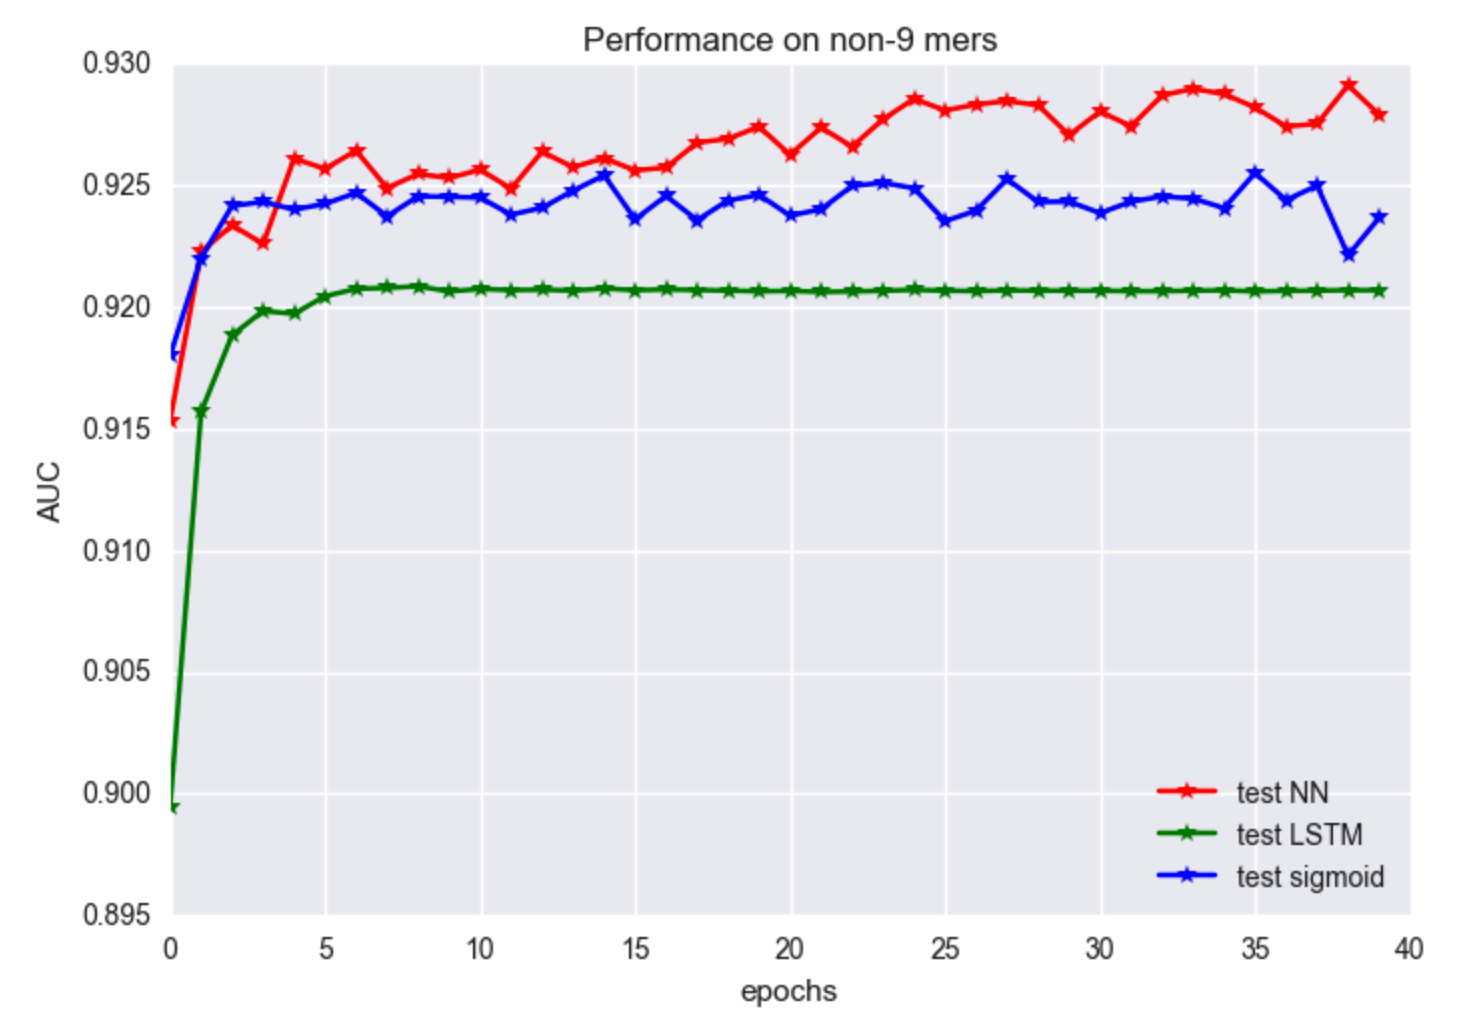
\includegraphics[scale = 0.17]{LSTM_vs_FFN_vs_sigmoid_non9mers.png}

Segmenting the test set into 9 mers and non 9 mers, one notices that the slightly inferior performance of the LSTM model stems mainly from its worse performance on non 9 mers, while both models perform about the same on 9 mers.\\

Quite surprisingly a simple sigmoid layer does a better job on non-9 mers than LSTM. This either means that kmer-index-encoding is doing particularly well on non-9 mers, or LSTM is doing particularly bad on non-9 mers.  
%=========================================================
\section{Convolutional Long Short-Term Memory models}
%=========================================================
In this section we present our new approach we adopted to increase the performance of the previous LSTM model. After embedding the index-encoded peptides, we perform one-dimensional convolutions with increasing filter sizes with 32 dimensional output and same padding on each amino acid positions. The maximal filter length being used coincides with the maximal peptide length across all alleles. For each amino acid position, we concatenate the one-dimensional convolutions column-wise, after which we concatenate the $26$ resulting $26*32$ long vectors row-wise. We have thus created a $26\times 26*32$ matrix which we feed row after row into the LSTM. 

Again three-fold cross validation on the training set was used to select the hyper-parameters. We selected the following model:
\begin{itemize}
  \item batch size of 16	
  \item 32 output dimensions for the amino acid vector embedding
  \item the hidden layer size of the LSTM being $50$
  \item the highest leverage parameter for regularization is the W dropout probability, which we set to $0.75$. W dropout is the dropout parameter associated with the weight matrix W multiplying the input vectors at each timestep. 
  \item the concatenated outputs are followed by a single dense sigmoid output with dropout rate $0.25$.
  \item Adaptive Moment Estimation (Adam) as optimization procedure.
  \item we have not imposed any learning rate decay as the model keeps improving significantly on non 9 mers.
\end{itemize}

We have found that in this case a bidirectional LSTM or stacked LSTMs instead of single LSTM does not improve the performance.  Here the cross-validation performance of the allele HLA-A0201:

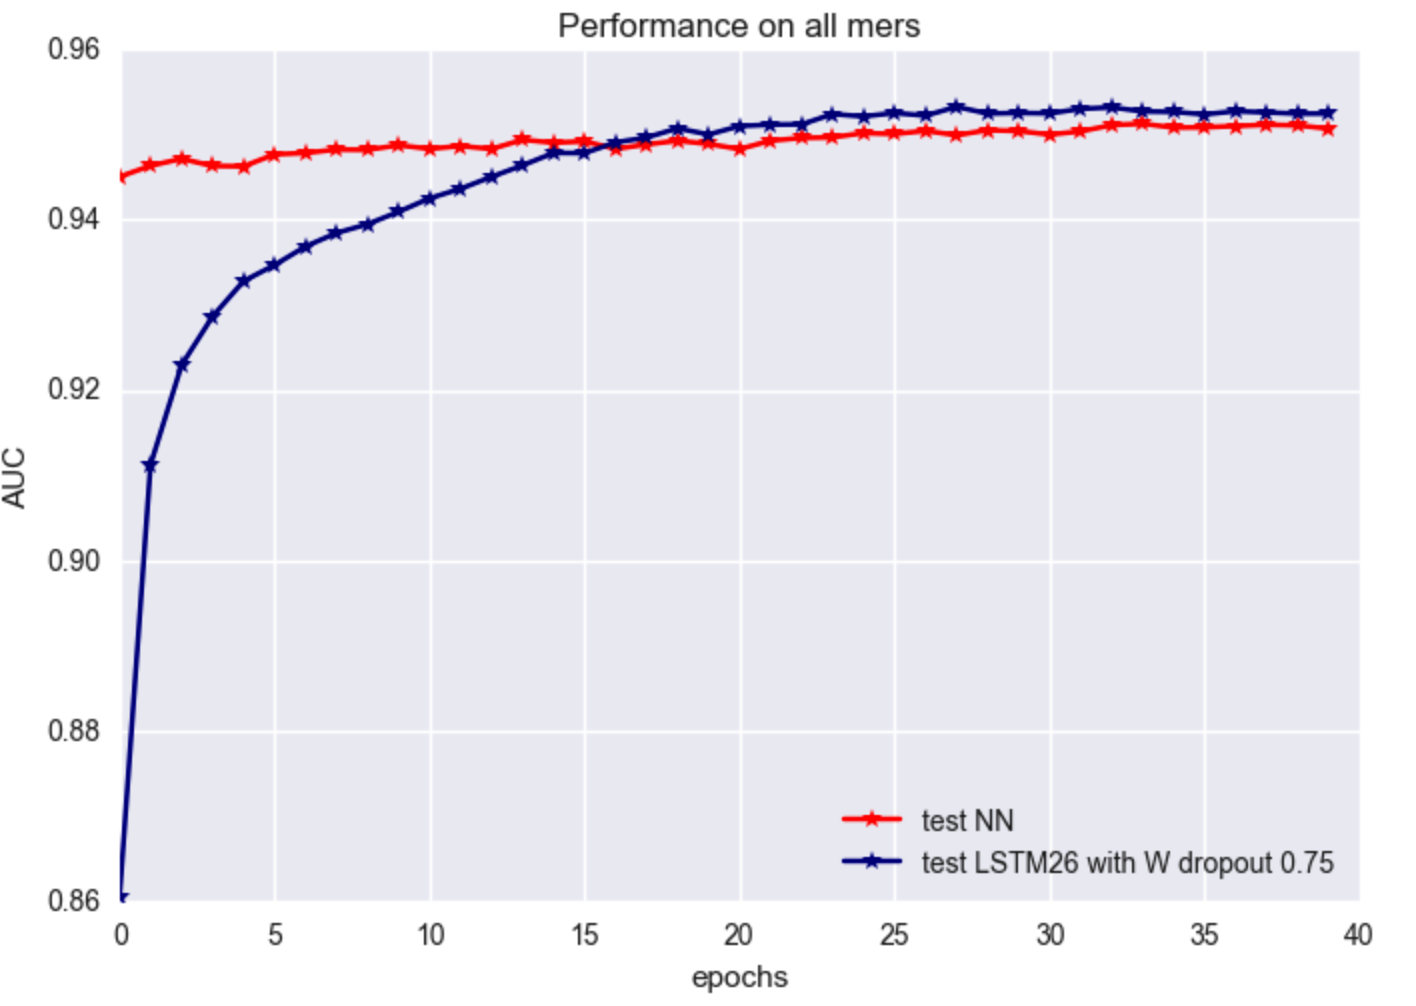
\includegraphics[scale = 0.17]{convLSTM_vs_FFN.png}
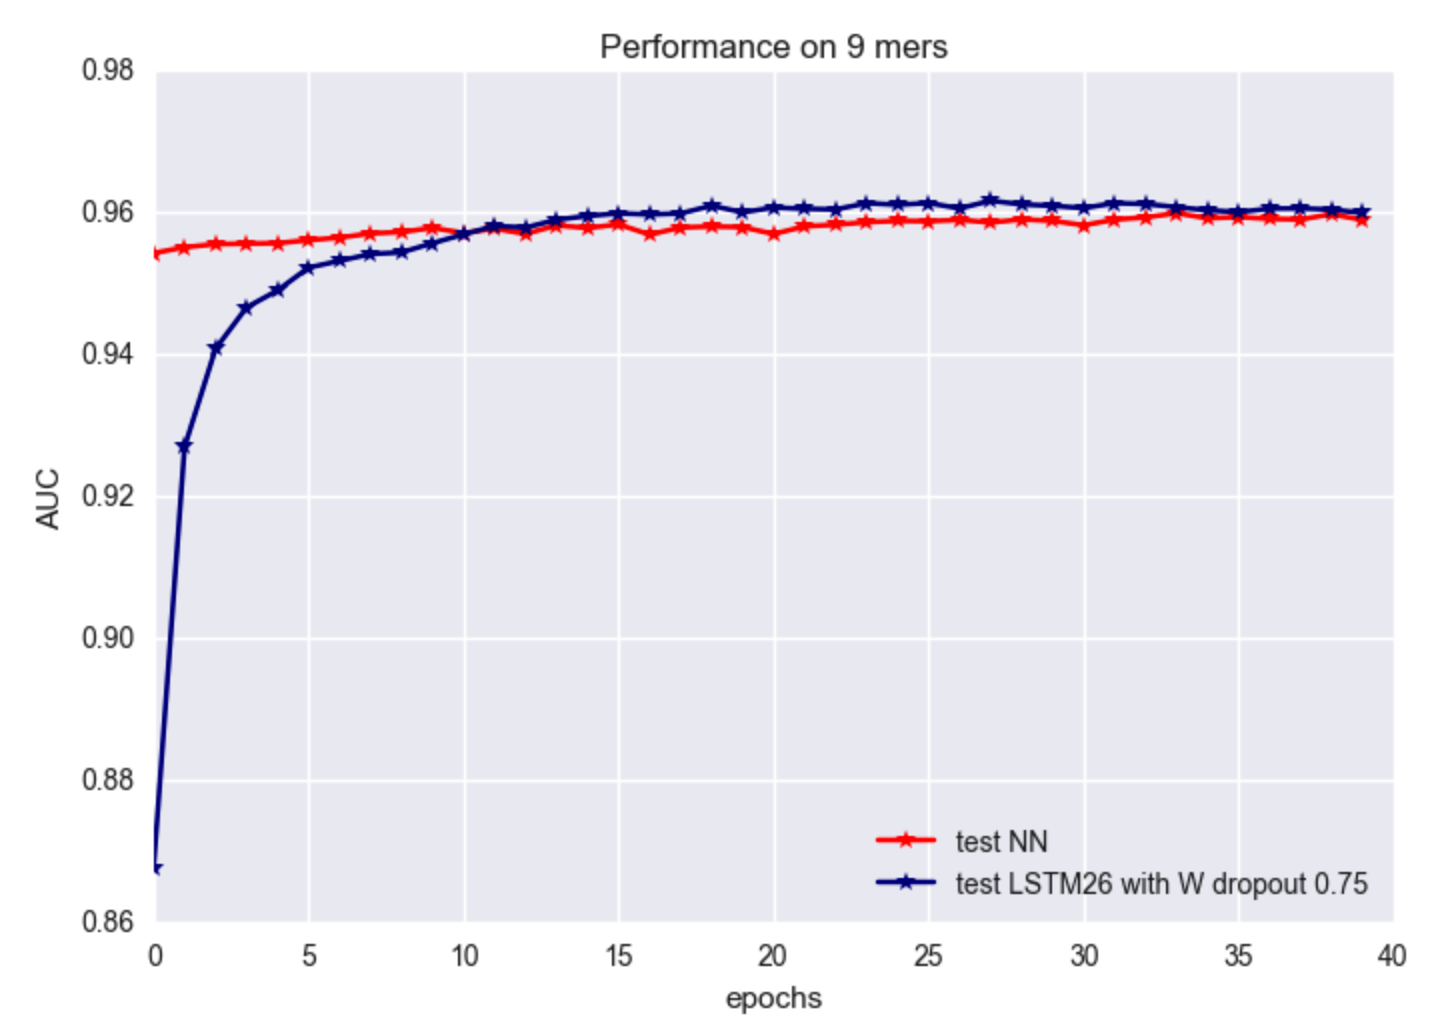
\includegraphics[scale = 0.17]{convLSTM_vs_FFN_9mers.png}
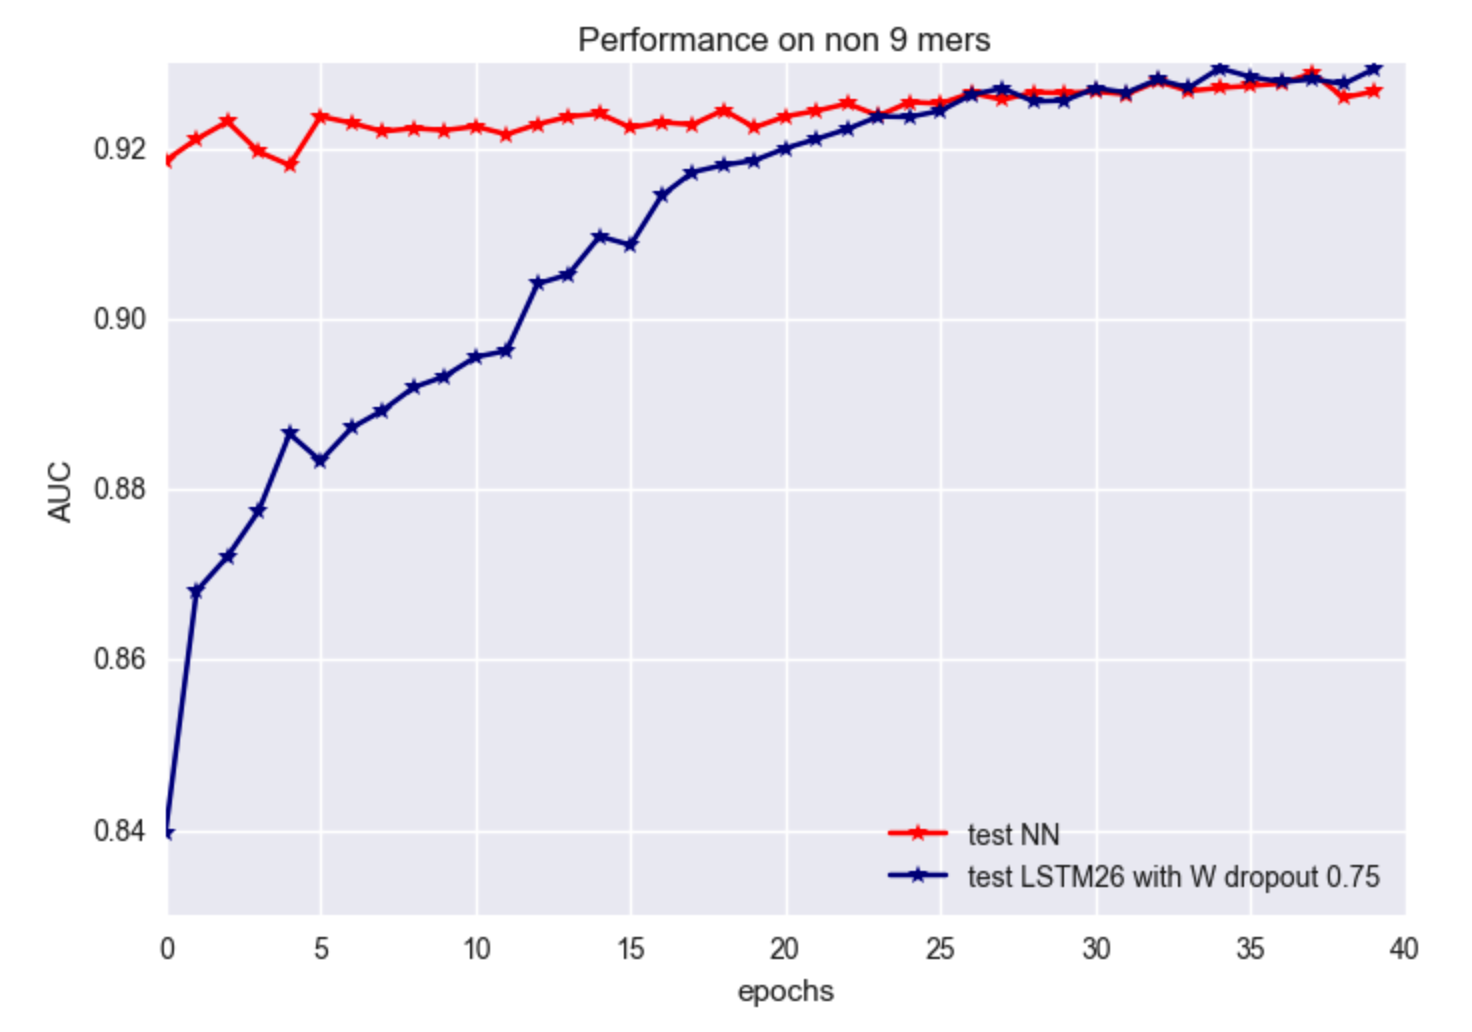
\includegraphics[scale = 0.17]{convLSTM_vs_FFN_non9mers.png}


The reason we believe the performance is superior to a simple LSTM model without convolution is because at each time-step the LSTM reads a vector not only containing the amino acid information but also the information of the amino acids surrounding it, thus giving rise to more contextual information within the peptide.

%=========================================================
\begin{small}
\setlength{\bibsep}{0.03cm}
%\bibliographystyle{abbrv}
\bibliographystyle{ieeetr}
%\bibliographystyle{apa}
\begin{thebibliography}{1}
\bibitem{cit1} Kim, Yohan et al. 'Immune Epitope Database Analysis Resource.' Nucleic Acids Research 40.Web Server issue (2012): W525?W530. PMC. Web. 13 Dec. 2016.
\bibitem{cit2} Greff, Klaus; Srivastava, Rupesh Kumar; Koutn�k, Jan; Steunebrink, Bas R.; Schmidhuber, J�rgen 'LSTM: A Search Space Odyssey' eprint arXiv:1503.04069
\bibitem{Kim_2014} Yohan Kim and John Sidney and S{\o}ren Buus and Alessandro Sette and Morten Nielsen and Bjoern Peters, 'Dataset size and composition impact the reliability of performance benchmarks for peptide-{MHC} binding predictions', BMC Bioinformatics
\bibitem{Salimi_2012} Nima Salimi and Ward Fleri and Bjoern Peters and Alessandro Sette, 'The immune epitope database: a historical retrospective of the first decade', Wiley-Blackwell, Immunology

\end{thebibliography}
\end{small}
%=========================================================





\end{document}

\grid
